\section{Introduction}

\begin{itemize}

\item What is the subject of the study? Describe the
economic/econometric problem.

-> Implementation of Cancer Gene Panels & Variant Calling Algorithms

\item What is the purpose of the study (working hypothesis)?

-> Check whether one of them is better than the others.
-> Study effect of FFPE

\item What do we already know about the subject (literature
review)? Use citations: { \cite{mutect:2013} shows that...
Alternative Forms of the Wald test are considered
\citep{Breusch&Schmidt:88}.}

\item What is the innovation of the study?

-> relatively rare technique in diagnostics, but has many advantages

\item Provide an overview of your results.


\end{itemize}

Cancer is a major public health problem worldwide and one of the leading death
causes. In 2012, there were an estimated 14.1 million new cancer cases with
estimated  8.2 million cancer deaths {\cite{cancer_stats_worldwide:2012}}. Lung
cancer is the most common cancer, both in terms of new cases (1.8 million) and
deaths (1.6 million). Breast  cancer is the second most common cancer (1.7
million cases) but only ranks 5th as cause of death (522,000 deaths). Colorectal
cancer (1.4 million cases; 694,000 deaths), prostate cancer (1.1 million cases;
307,000 deaths), stomach cancer (951,000 cases; 723,000 deaths) and liver cancer
(782,000 cases; 723,000 deaths) are following.

In Luxembourg, there were 1164 death cases caused by cancer in 2014, accounting
for 30.6\%  of the number of deaths. Cancer is thereby the second most common
death cause in Luxembourg, ranging behind cardiovascular diseases (1189 deaths;
31.3\%). Amongst these cancer deaths, cancers of the digestive organs (340
deaths) and of the respiratory organs (272 deaths) were the most frequent ones.
{\cite{cancer_stats:2012}}.

(Considerable effort is made by the research
community to understand the underlying causes of cancer and its progression, but
death rate related to cancer remains high. In Luxembourg, the death rate did not
significantly drop from 1998 to 2014.)

In recent years, more targeted drugs. personalized medicine.

Next-Generation Sequencing (NGS) is a powerful method to analyze RNA or DNA
molecules. Improved protocols and methods have been developed in recent years
that allow to implement NGS for a variety of applications in both research and
diagnostics. NGS is still hard to implement and is mainly used in research. Only
a few laboratories are using this technique as a diagnostic technique.The SGMB
is building expertise in NGS and is implementing targeted NGS in its molecular
pathology laboratory. This implementation aims at gaining deep insights into the
underlying causes of solid tumors and in guiding targeted cancer therapy.

The goal of this master's thesis was to compare commercially available cancer
gene panels on samples of solid tumor patients by several parameters and by
their ability to detect variants, which have previously been detected in the
routine mutation detection workflow in the laboratory. As a second part, several
freely available variant calling algorithms were compared for their potential
implementation in the custom in-house variant detection bioinformatic pipeline.

\subsection{EGFR Signaling in Cancer}

Bla {\cite{targeting_egfr:2012}}

Describe pathway

\begin{figure}[ht]
  \begin{center}
    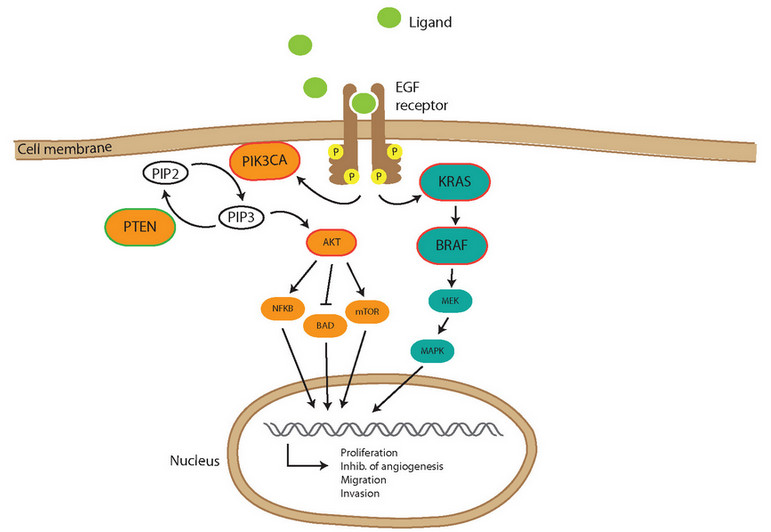
\includegraphics[scale=1,angle=0]{egfr_signaling.png}
    \caption{Schematic representation of the EGFR signaling cascade {\cite{targeting_egfr:2012}}}
    \label{Fig:egfr_signaling}
  \end{center}
\end{figure}

Common mutations in this pathway

EGFR-targeted drugs

\subsection{Targeted Sequencing and Target Enrichment Methods}

{\cite{enrichment_methods:2011}}

Hybrid capture

Selective circularization

PCR amplification

\subsection{Illumina MiSeq Sequencing Chemistry}

Picture

\subsection{NGS Data Analysis}

GATK best practices

\subsection{Practical Implications in the Laboratory}

FFPE : more details

\subsection{Aims of the Thesis}
Targeted NGS is still not widely used in diagnostics laboratories. The SGMB of the LNS
is planning to build expertise with the aim to adopt NGS routinely in the laboratory,
mainly in the context of diagnosis and therapy of cancer patients in Luxembourg.

The aim of this thesis project was to test commercially available cancer gene panels,
e.g. Illumina Trusight Tumor 15 and Agilent Haloplex HS ClearSeq Cancer, for their
potential use in the routine workflow of the laboratory. Several samples of cancer
patients were prepared with both kits and were sequenced on the Illumina MiSeq device.
Both kits vary in their sequencing library preparation principles: Illumina's tst15
uses the multiplex PCR approach while Agilent's Haloplex Enrichment System uses
enzymatic DNA restriction followed by probe capture.

NGS data were analyzed with the respective recommended pipelines and a custom in-house
pipeline.

Finally, several freely available variant calling algorithms were tested for their
potential implementation in the custom in-house variant discovery bioinformatic
pipeline.
